\chapter{Observatory}

This chapter explains how to use the Observatory application.

\section{Homepage}

Figures \ref{fig:obs_homepage} - \ref{fig:obs_homepage_2}.

\begin{figure}[H]
    \centering
    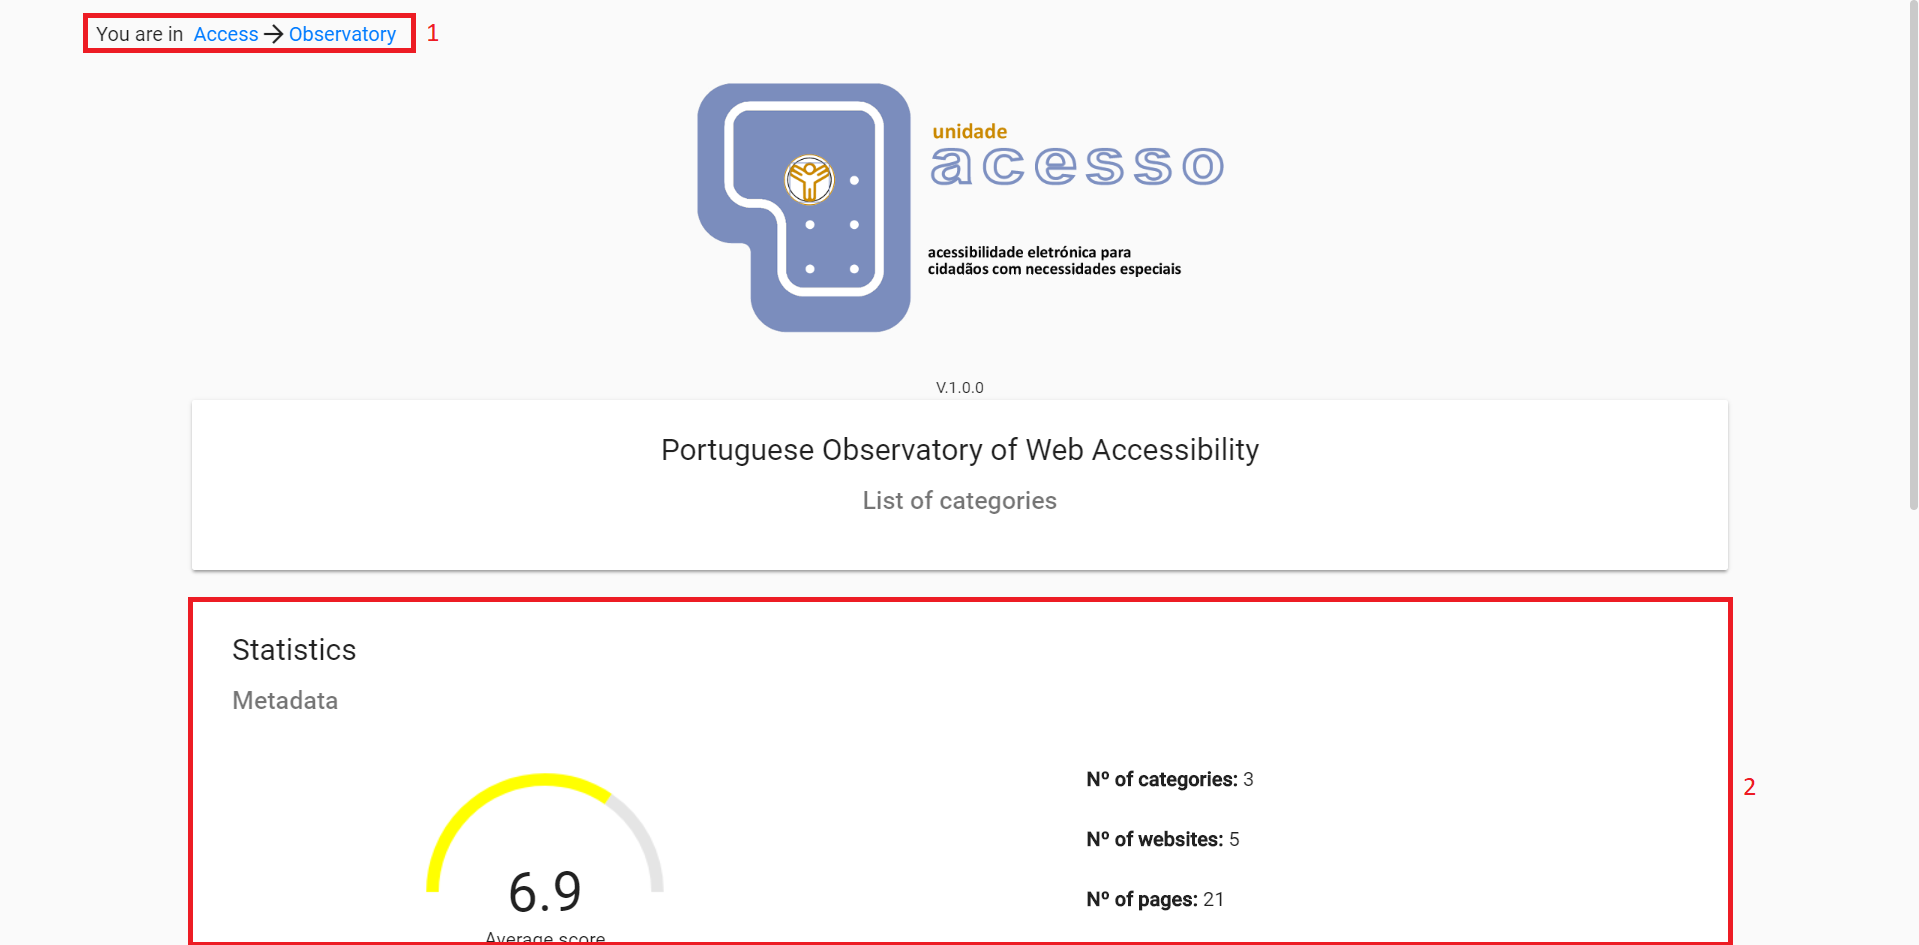
\includegraphics[width=\linewidth]{lib/images/observatory/observatory_homepage.png}
    \caption{Observatory homepage}
    \label{fig:obs_homepage}
\end{figure}

\clearpage

\begin{figure}[H]
    \centering
    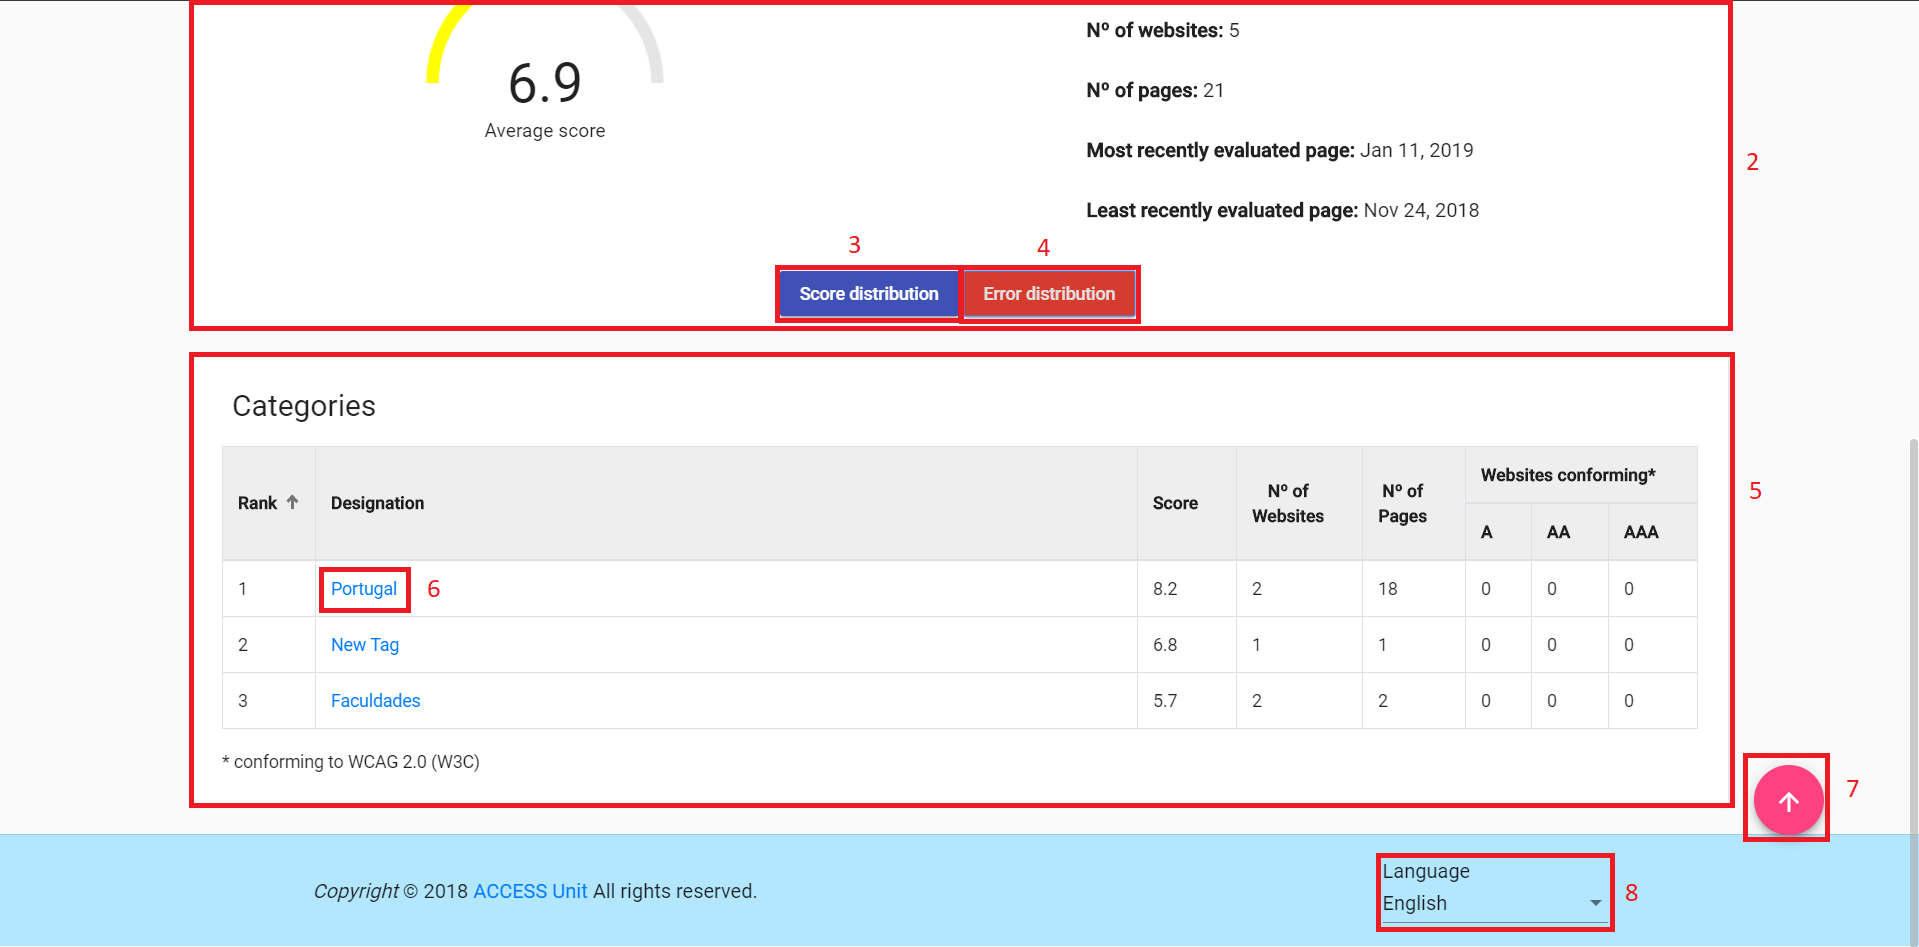
\includegraphics[width=\linewidth]{lib/images/observatory/observatory_homepage_2.png}
    \caption{Observatory homepage (cont.)}
    \label{fig:obs_homepage_2}
\end{figure}

\begin{enumerate}
    \item Breadcrumbs menu
    \item List of all categories statistics
    \item See score distribution graph/table (example figures \ref{fig:obs_website_page_score_graph} - \ref{fig:obs_website_page_score_table})
    \item See error distribution graph/table (example figures \ref{fig:obs_website_page_error_graph} - \ref{fig:obs_website_page_error_table})
    \item List of categories
    \item See information about that specific category
    \item ``Go to top'' button
    \item Language selection box
\end{enumerate}

\clearpage

\section{Category page}

Figures \ref{fig:obs_category_page} - \ref{fig:obs_category_page_2}.

\begin{figure}[H]
    \centering
    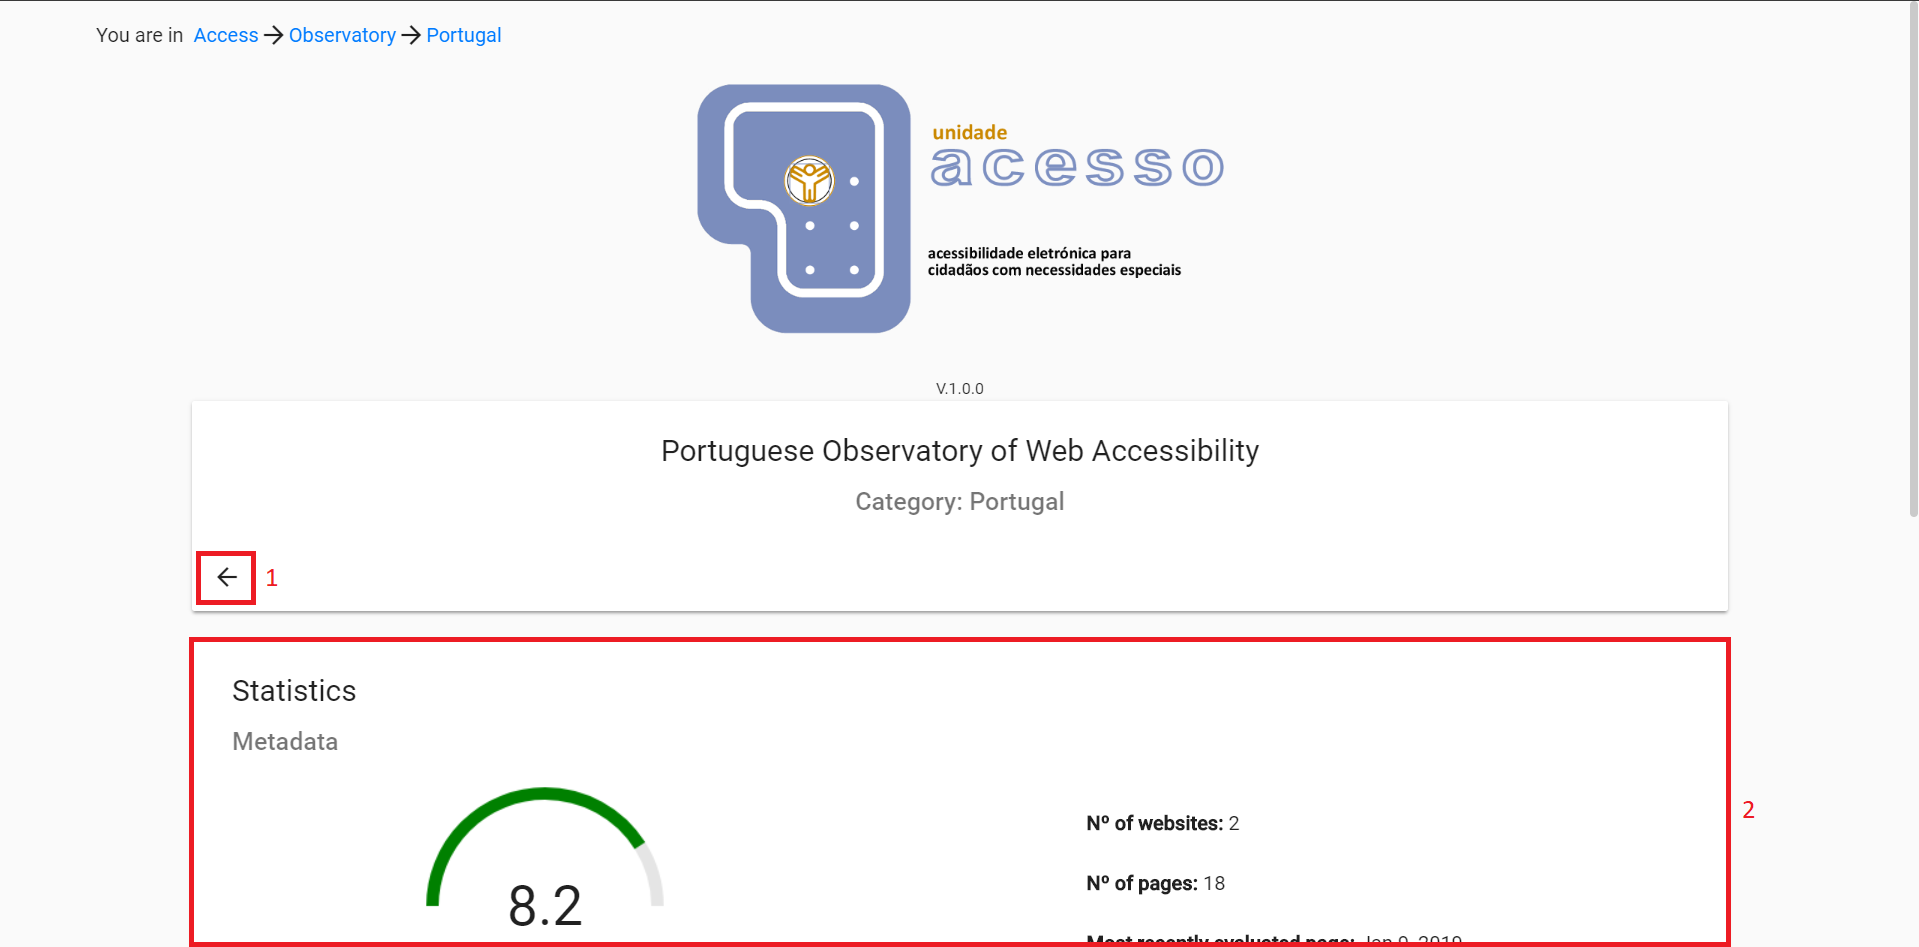
\includegraphics[width=\linewidth]{lib/images/observatory/observatory_category_page.png}
    \caption{Observatory category page}
    \label{fig:obs_category_page}
\end{figure}

\begin{figure}[H]
    \centering
    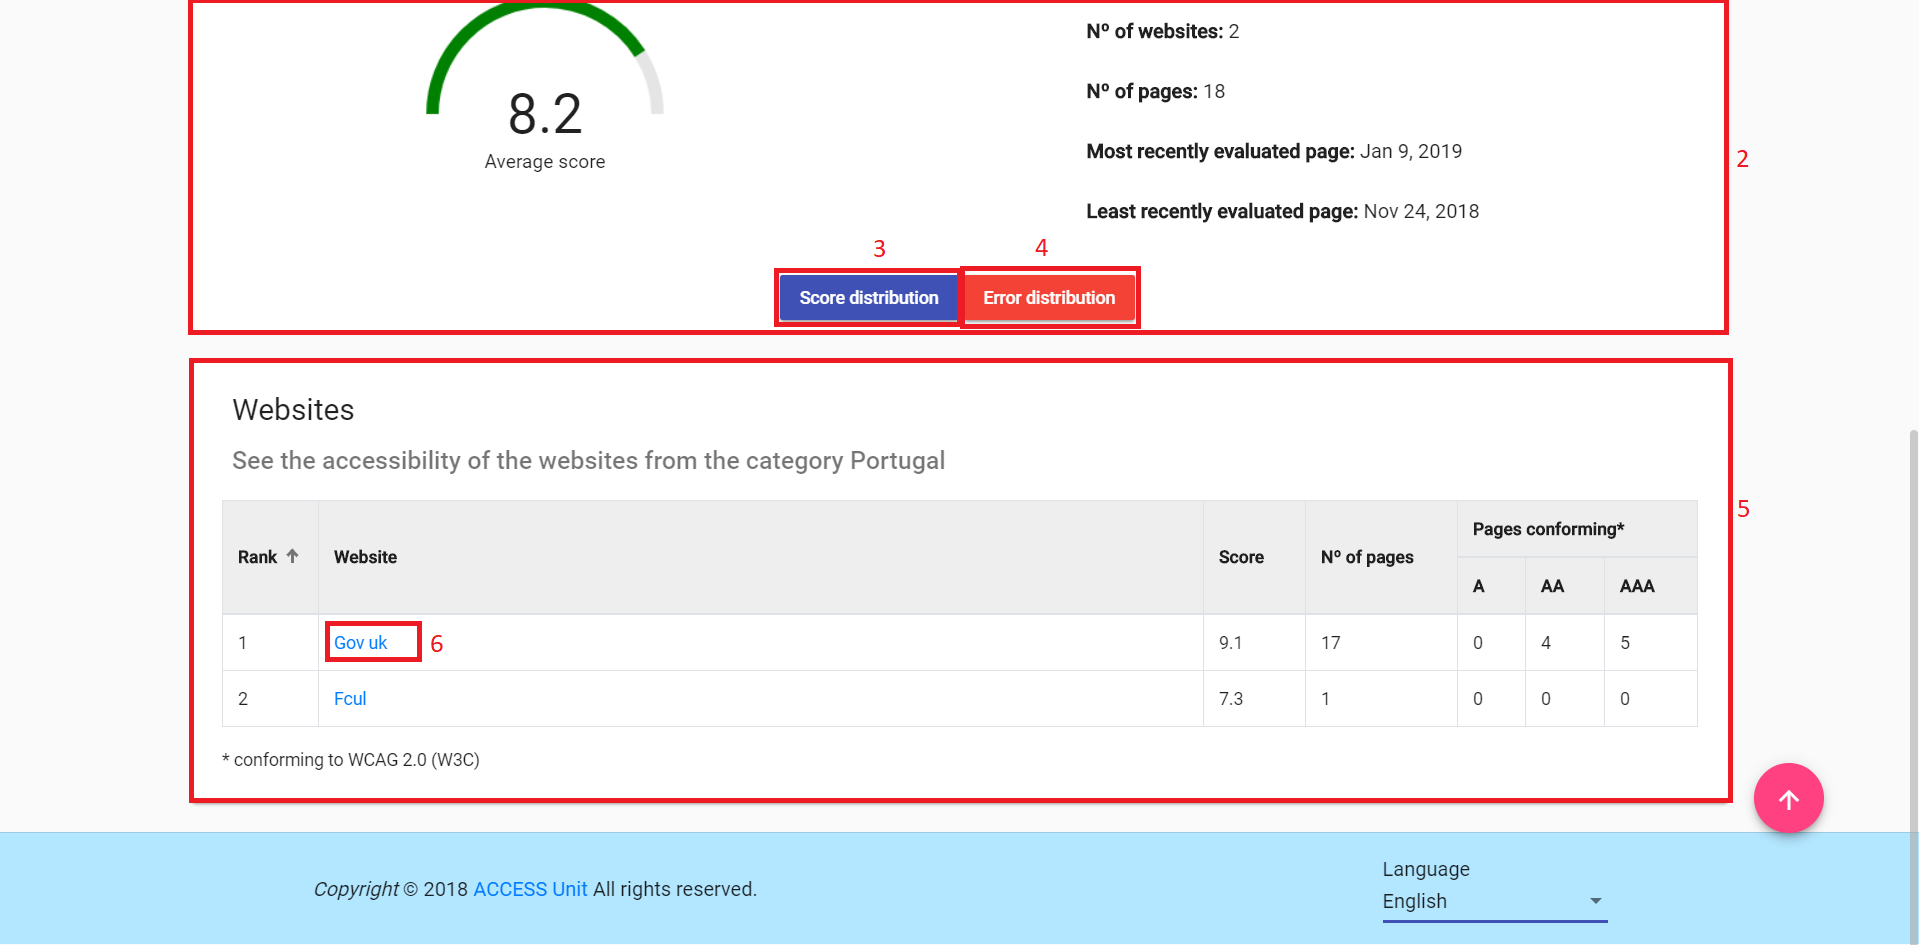
\includegraphics[width=\linewidth]{lib/images/observatory/observatory_category_page_2.png}
    \caption{Observatory category page (cont.)}
    \label{fig:obs_category_page_2}
\end{figure}

\begin{enumerate}
    \item Goes back to the previous page (homepage)
    \item Category statistics
    \item See score distribution graph/table (example figures \ref{fig:obs_website_page_score_graph} - \ref{fig:obs_website_page_score_table})
    \item See error distribution graph/table (example figures \ref{fig:obs_website_page_error_graph} - \ref{fig:obs_website_page_error_table})
    \item List of category websites
    \item See information about that specific website
\end{enumerate}

\clearpage

\section{Website page}

Figures \ref{fig:obs_website_page} - \ref{fig:obs_website_page_4}.

\begin{figure}[H]
    \centering
    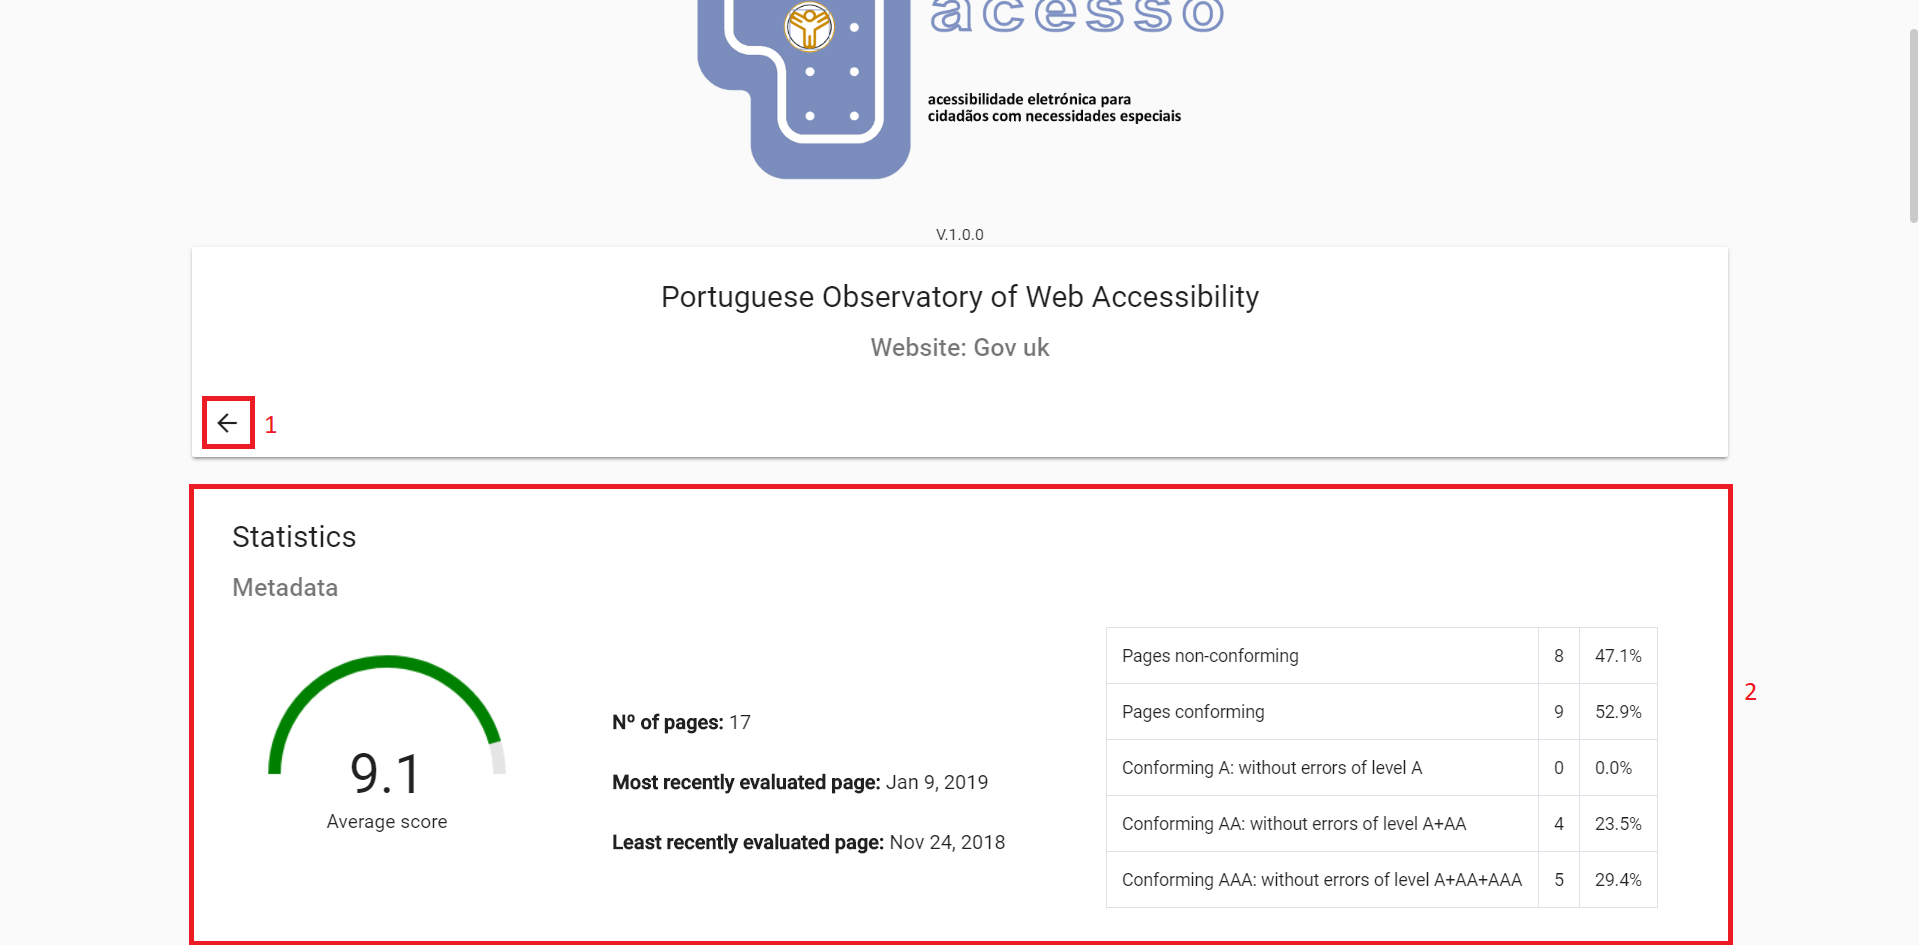
\includegraphics[width=\linewidth]{lib/images/observatory/observatory_website_page.png}
    \caption{Observatory website page}
    \label{fig:obs_website_page}
\end{figure}

\begin{figure}[H]
    \centering
    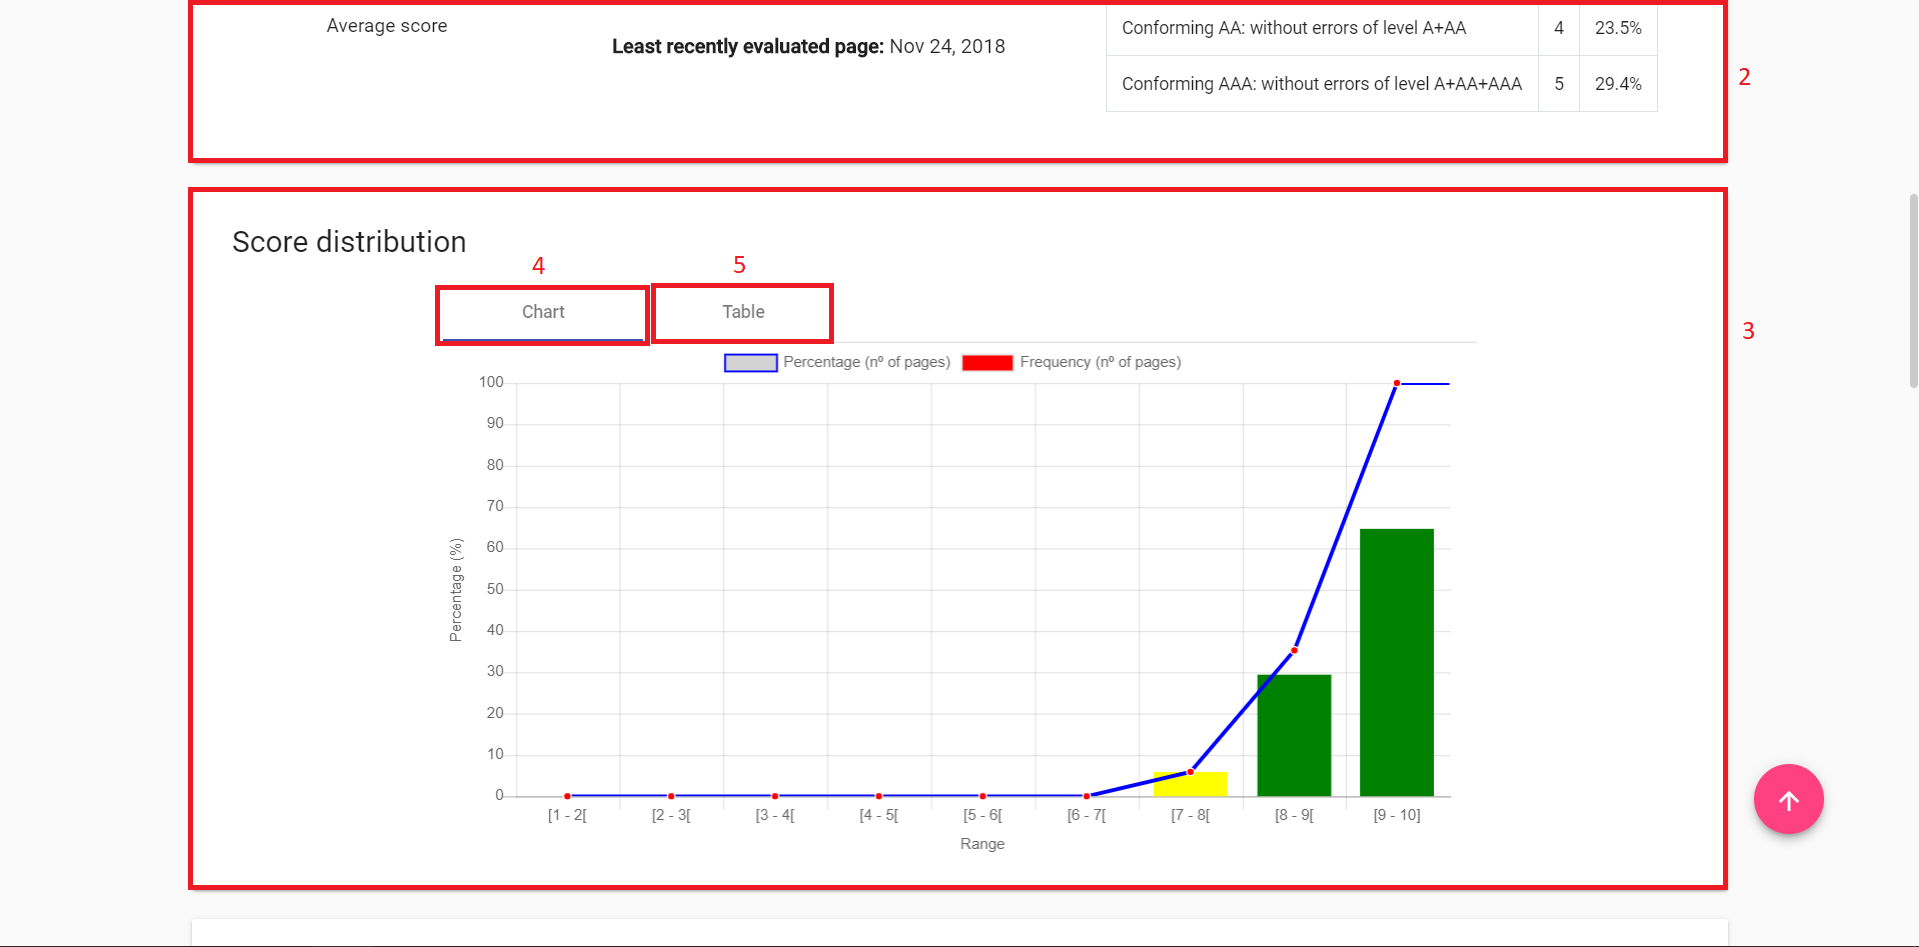
\includegraphics[width=\linewidth]{lib/images/observatory/observatory_website_page_score_graph.png}
    \caption{Observatory website page (cont.)}
    \label{fig:obs_website_page_score_graph}
\end{figure}

\begin{figure}[H]
    \centering
    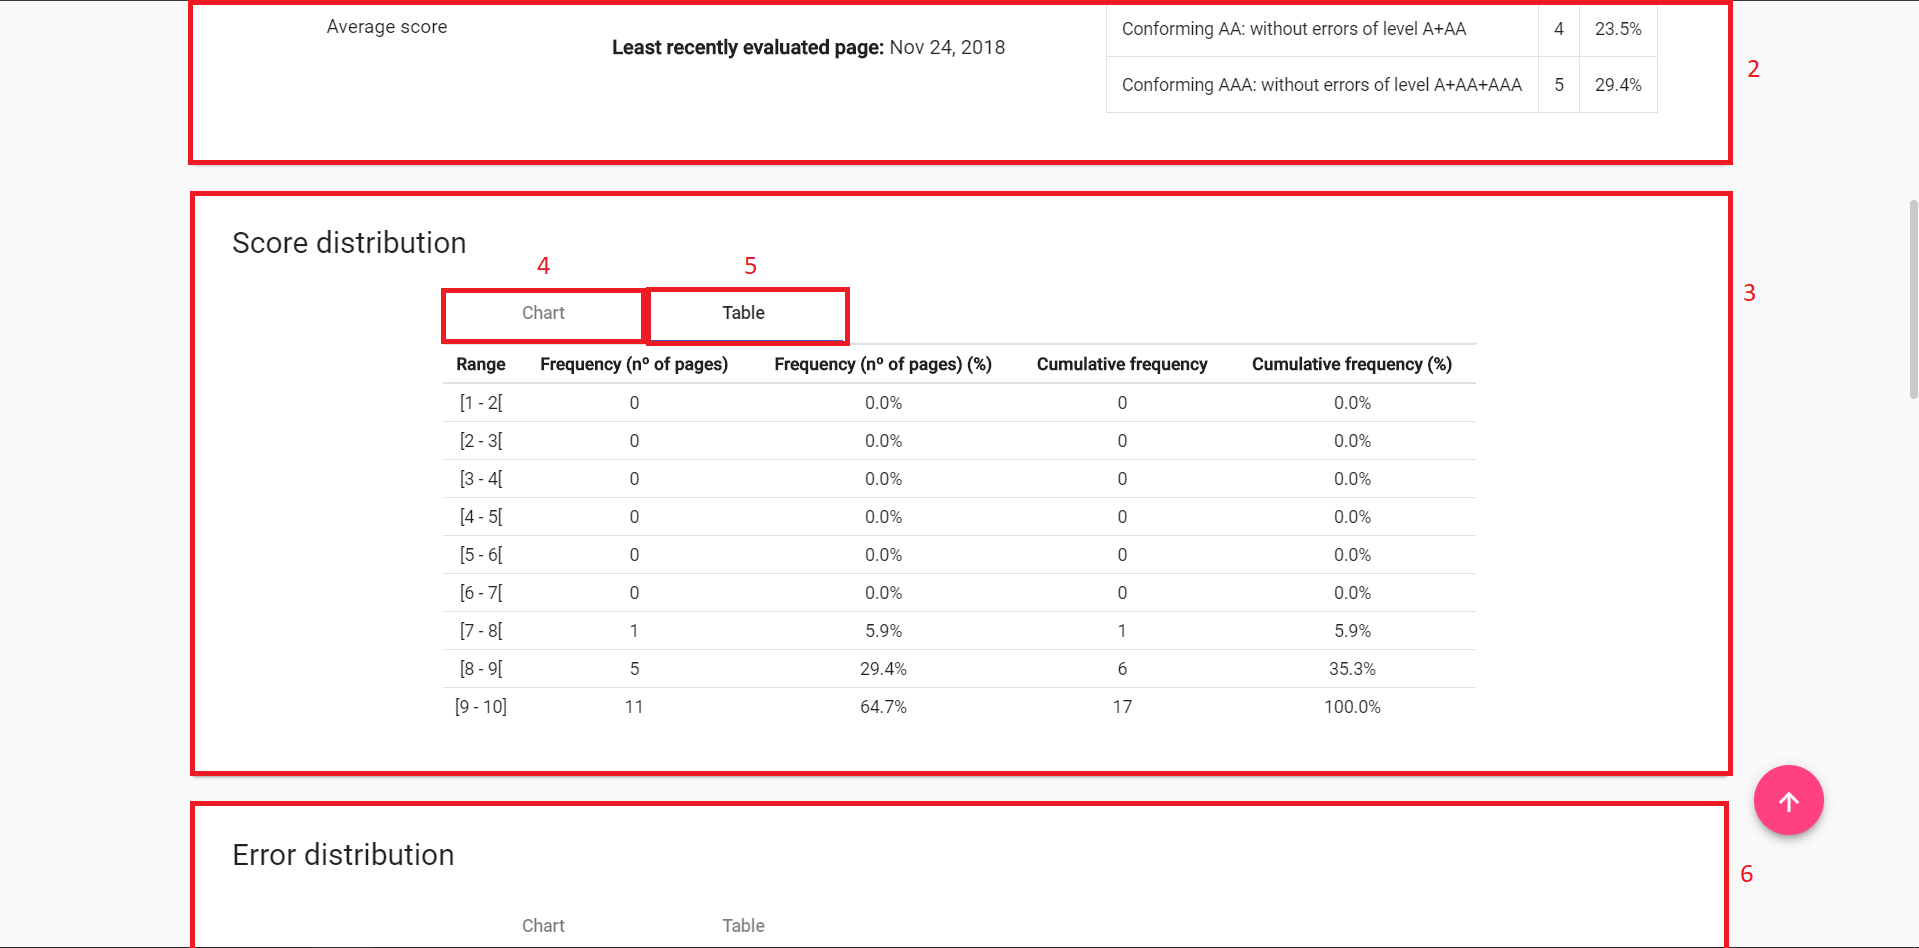
\includegraphics[width=\linewidth]{lib/images/observatory/observatory_website_page_score_table.png}
    \caption{Observatory website page (cont.)}
    \label{fig:obs_website_page_score_table}
\end{figure}

\begin{figure}[H]
    \centering
    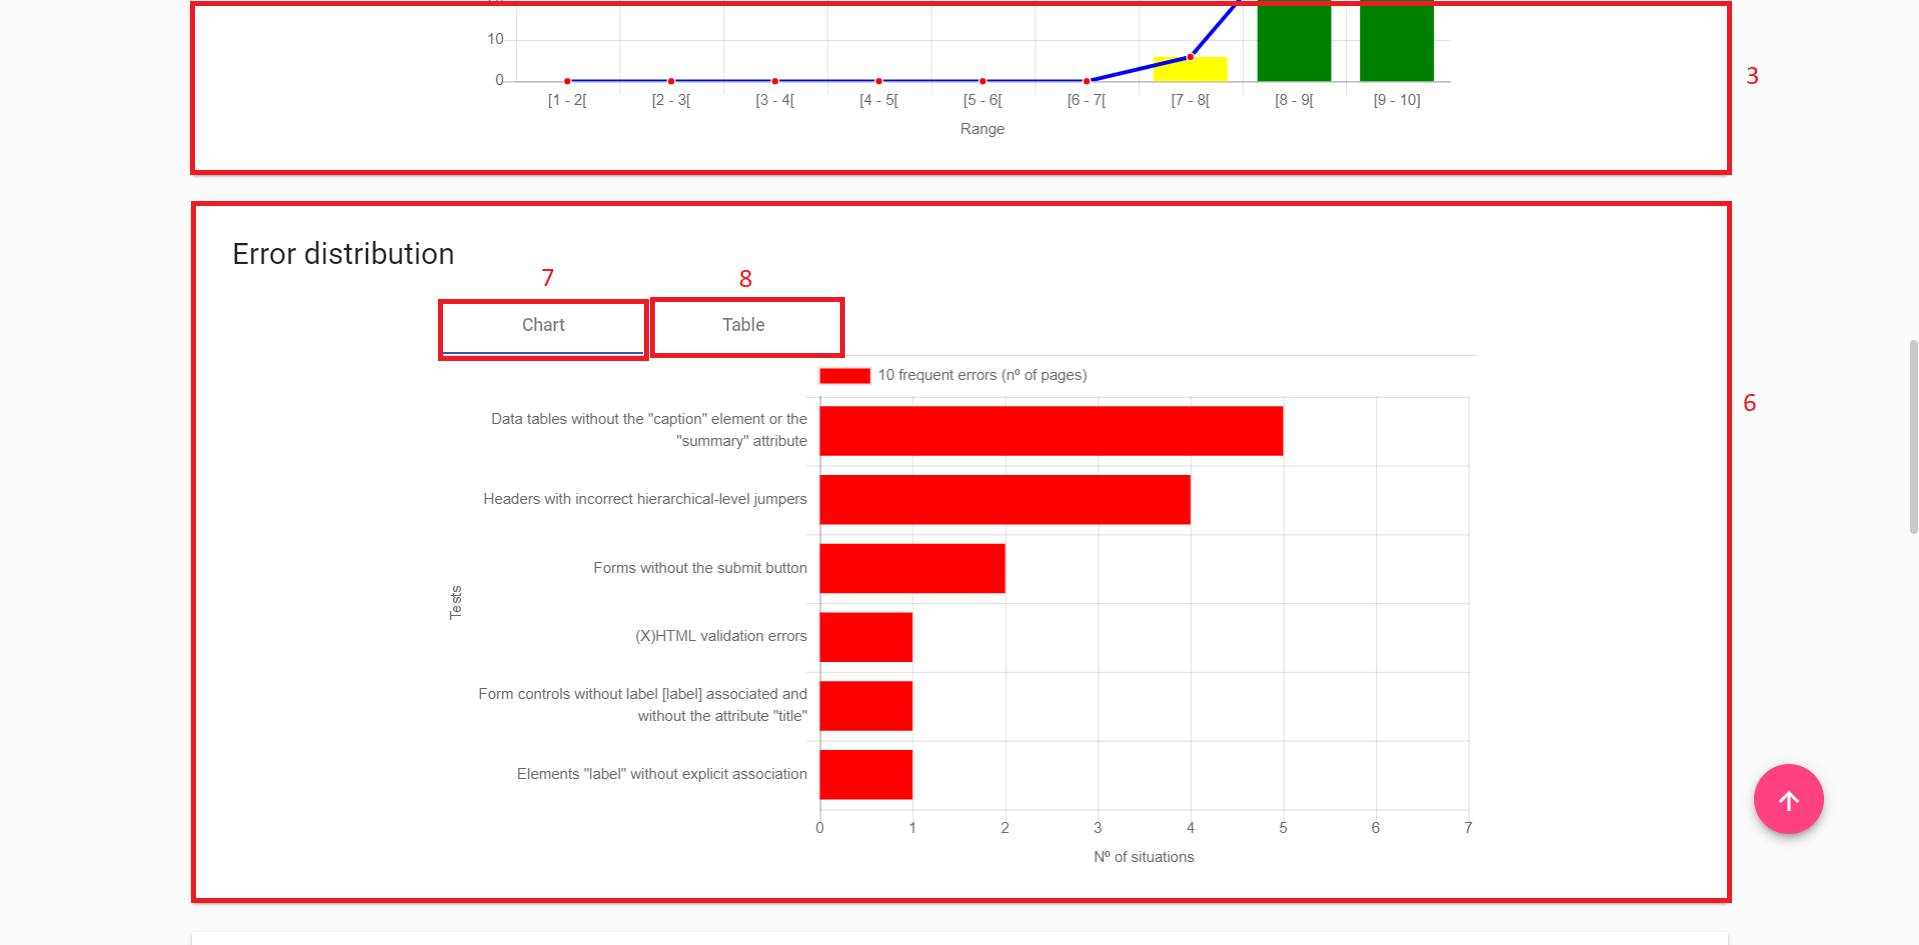
\includegraphics[width=\linewidth]{lib/images/observatory/observatory_website_page_error_graph.png}
    \caption{Observatory website page (cont.)}
    \label{fig:obs_website_page_error_graph}
\end{figure}

\begin{figure}[H]
    \centering
    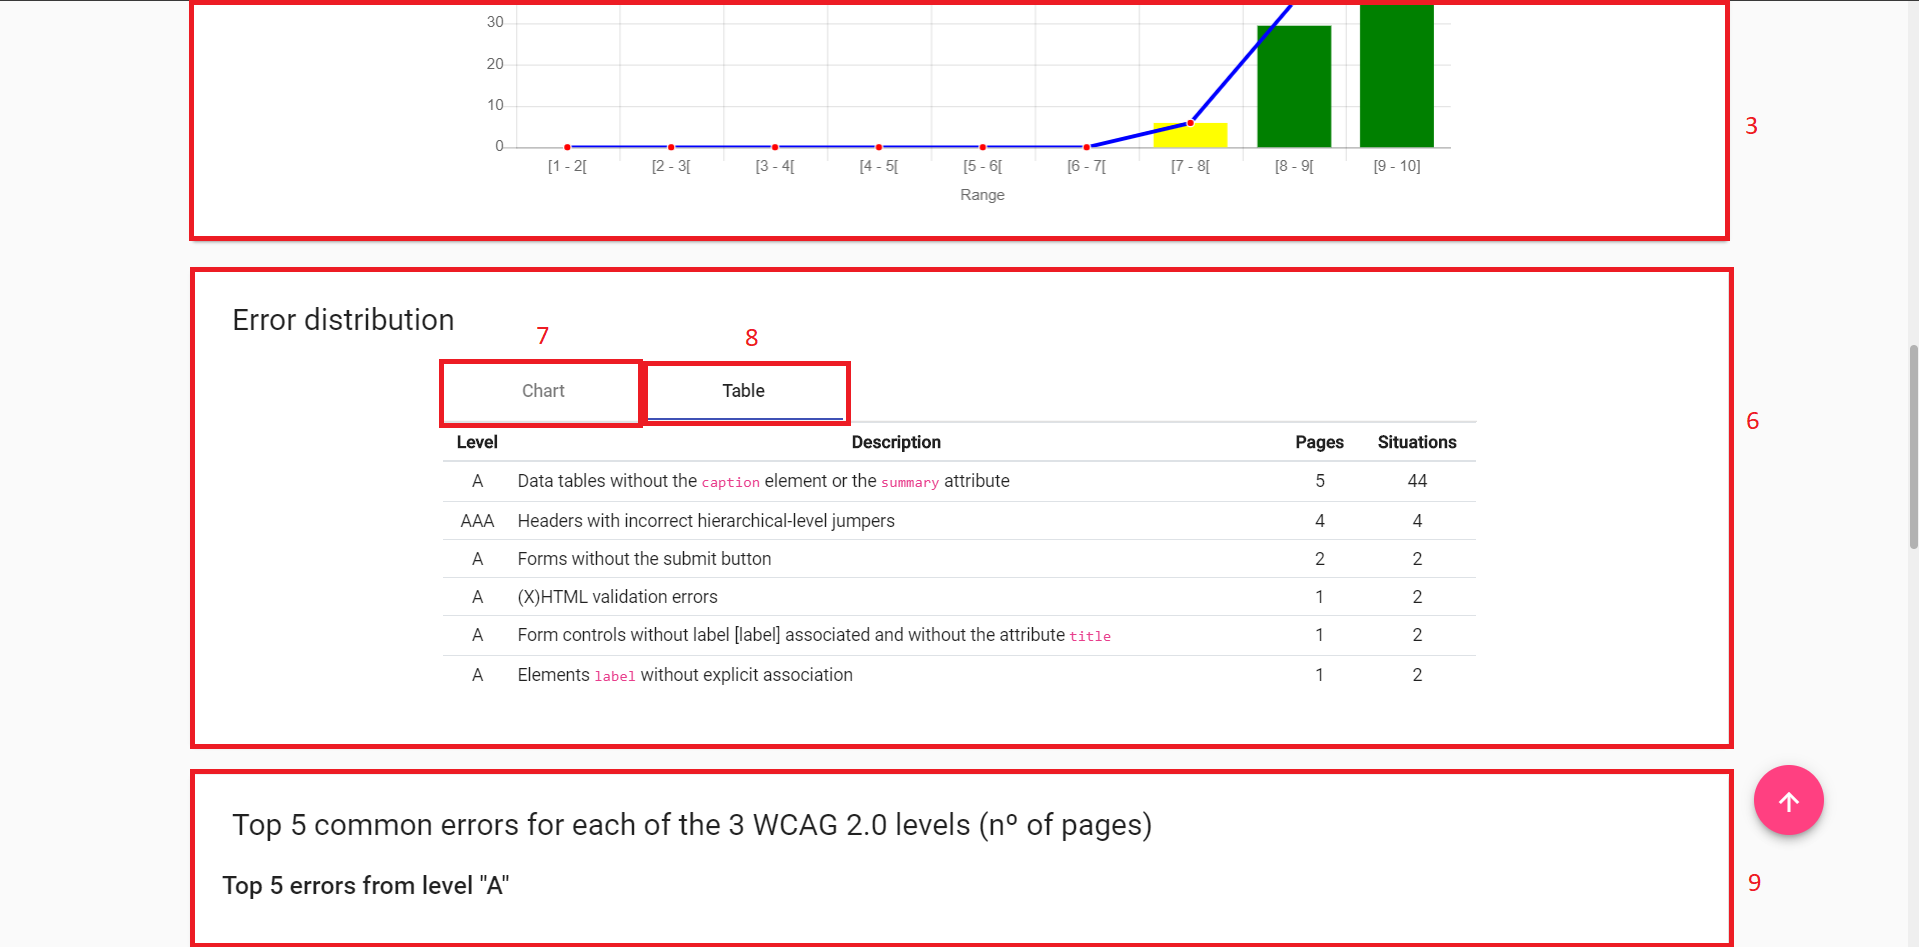
\includegraphics[width=\linewidth]{lib/images/observatory/observatory_website_page_error_table.png}
    \caption{Observatory website page (cont.)}
    \label{fig:obs_website_page_error_table}
\end{figure}

\begin{figure}[H]
    \centering
    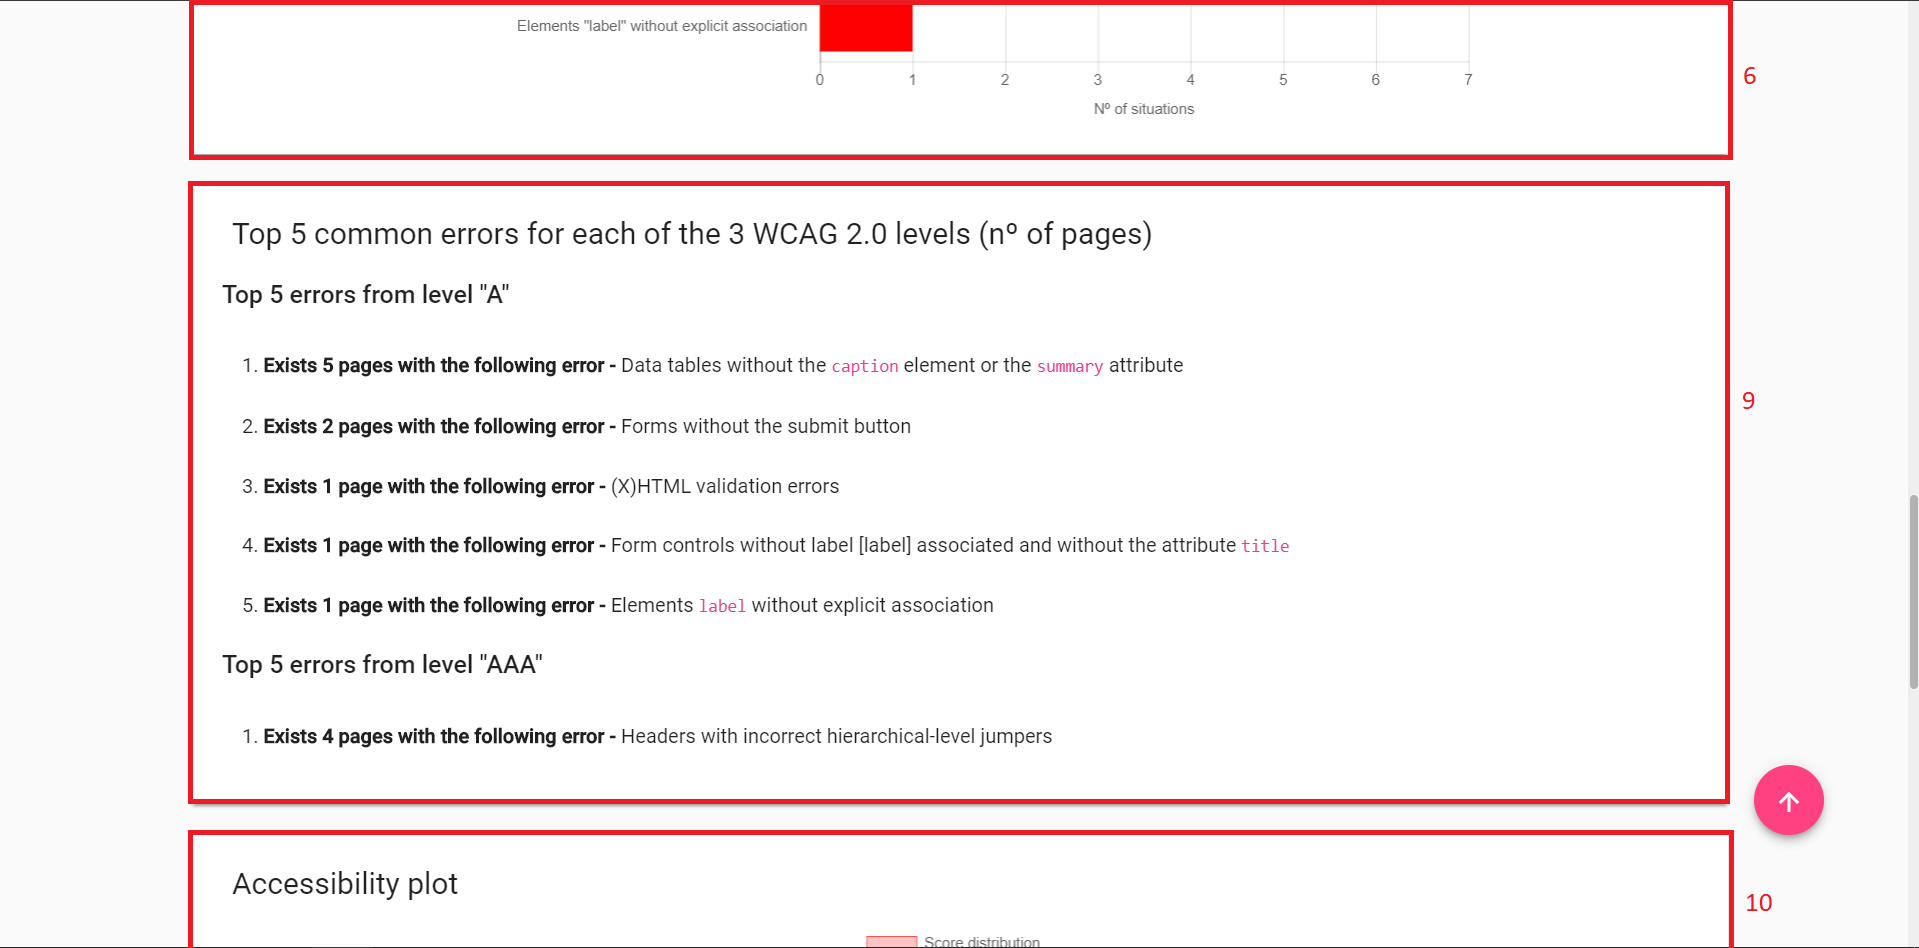
\includegraphics[width=\linewidth]{lib/images/observatory/observatory_website_page_2.png}
    \caption{Observatory website page (cont.)}
    \label{fig:obs_website_page_2}
\end{figure}

\begin{figure}[H]
    \centering
    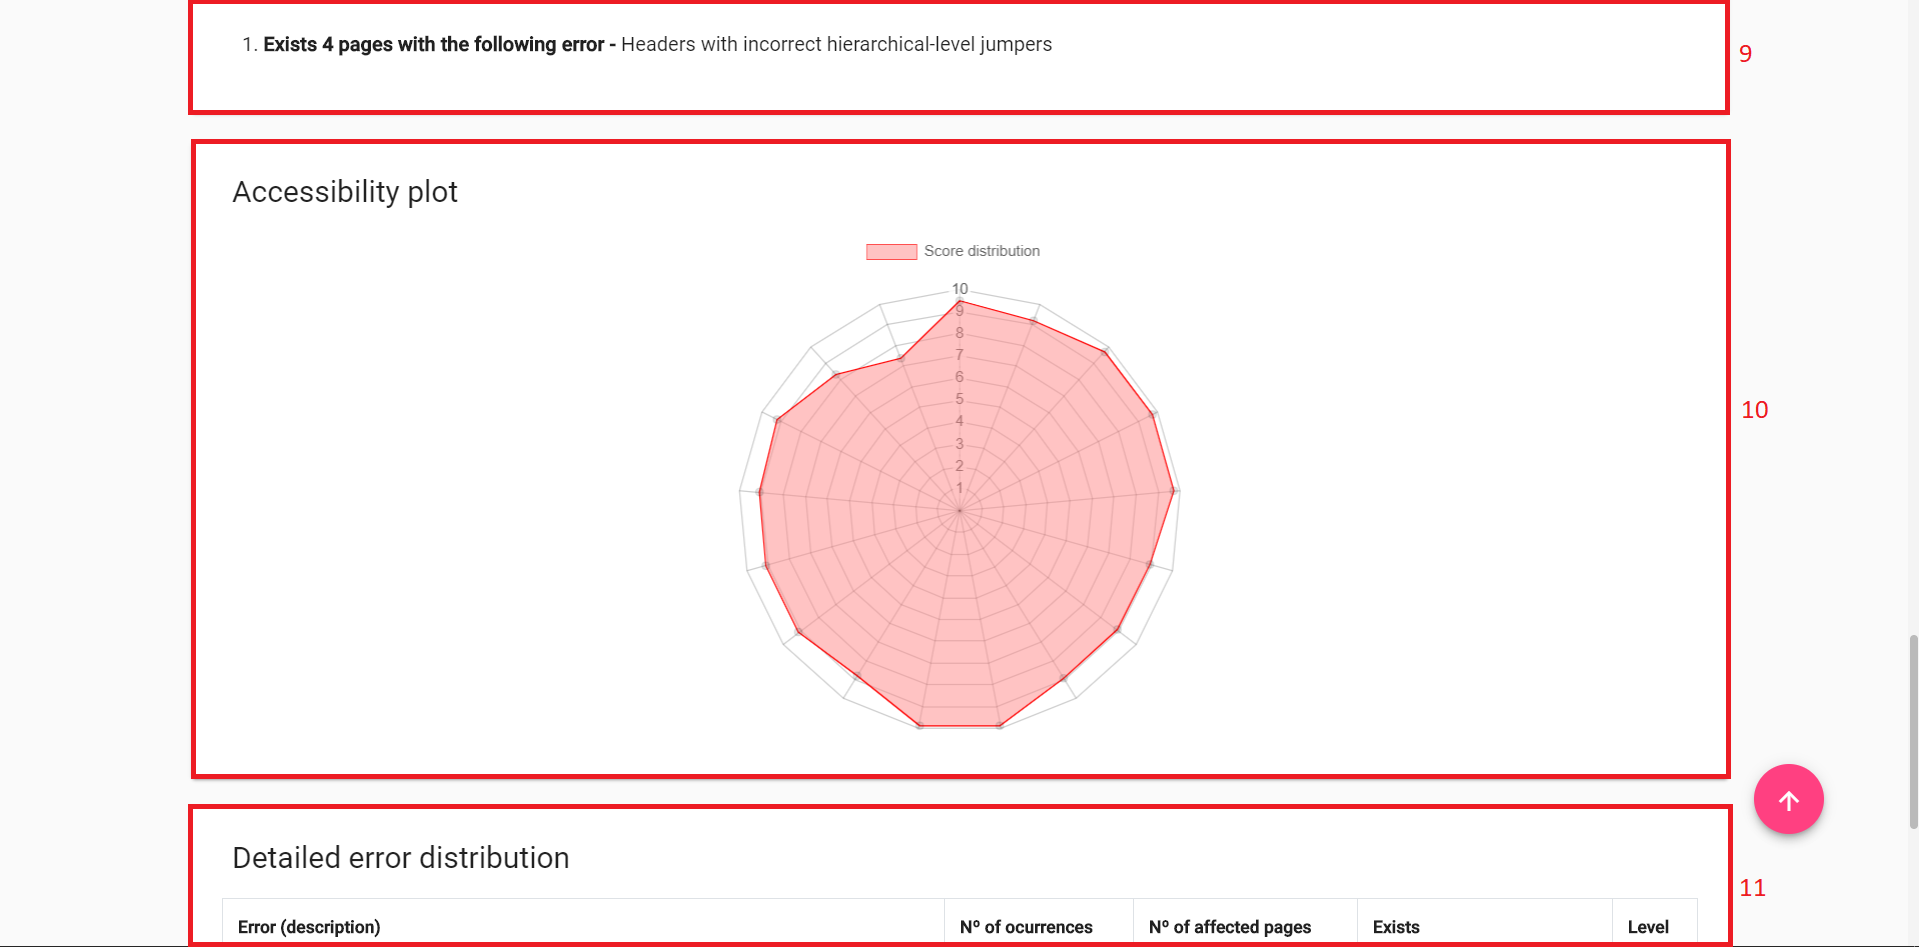
\includegraphics[width=\linewidth]{lib/images/observatory/observatory_website_page_3.png}
    \caption{Observatory website page (cont.)}
    \label{fig:obs_website_page_3}
\end{figure}

\begin{figure}[H]
    \centering
    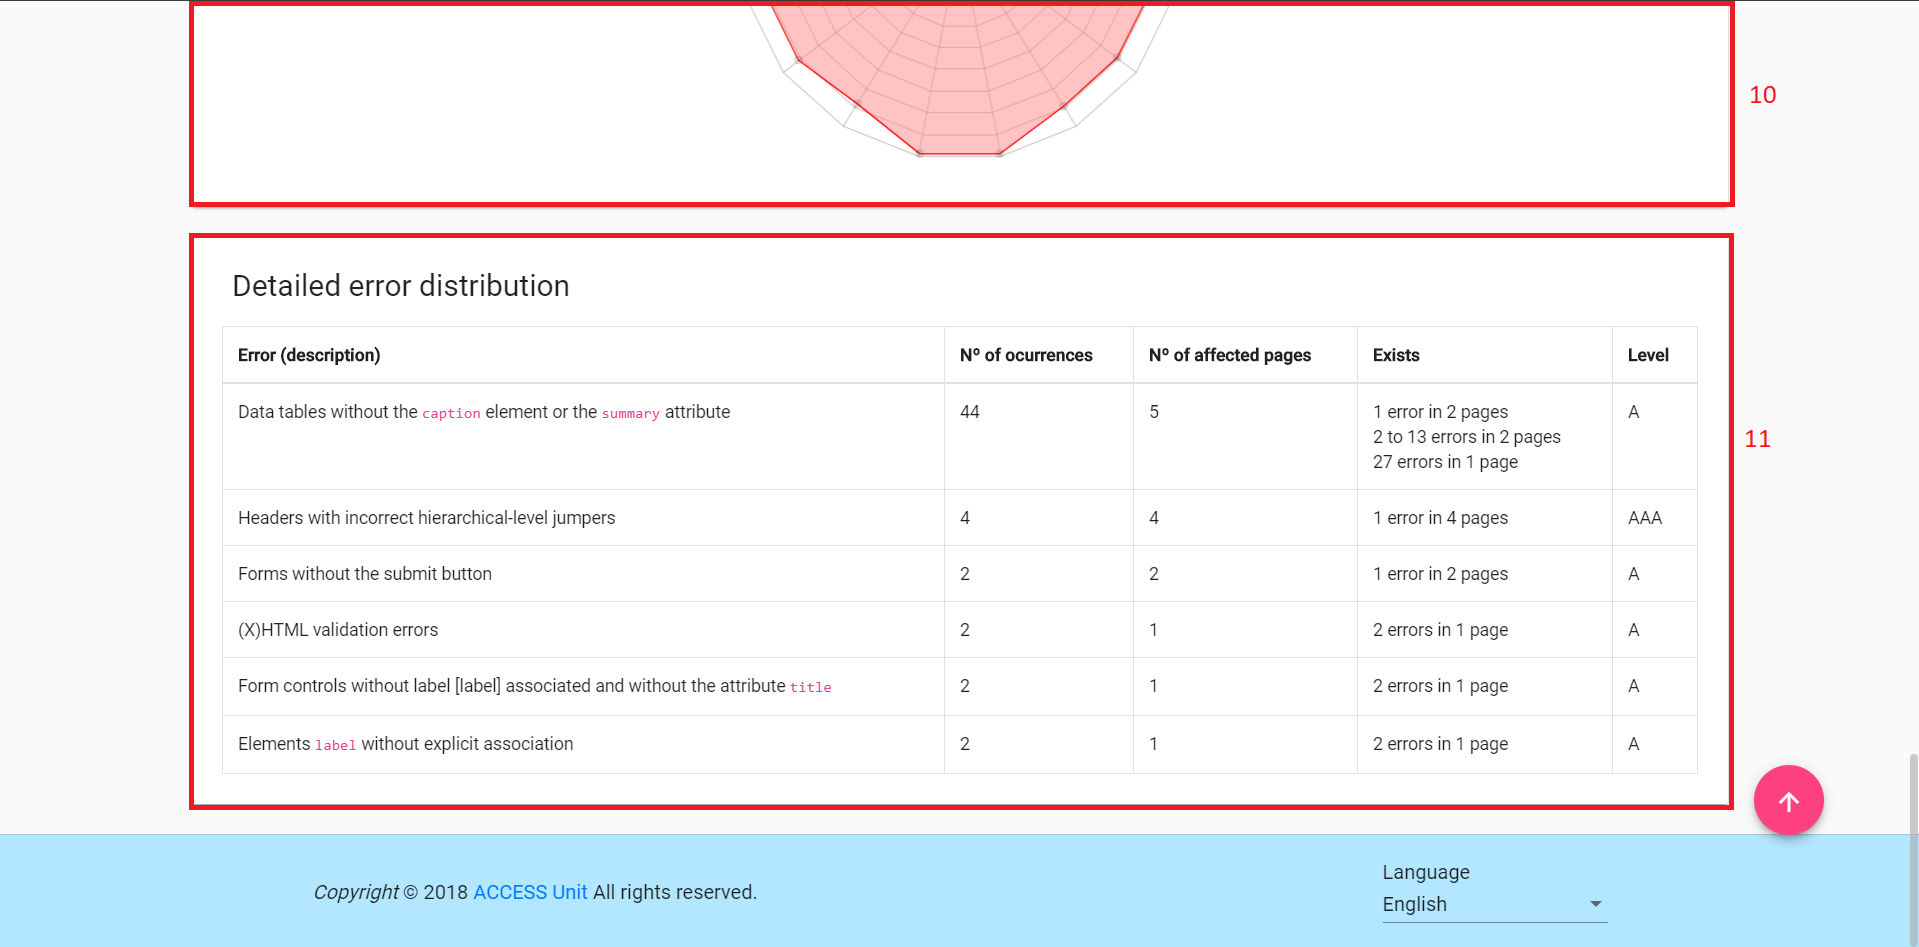
\includegraphics[width=\linewidth]{lib/images/observatory/observatory_website_page_4.png}
    \caption{Observatory website page (cont.)}
    \label{fig:obs_website_page_4}
\end{figure}

\begin{enumerate}
    \item Goes back to the previous page (category page)
    \item Website statistics
    \item Website score distribution
    \item See website score distribution graph
    \item See website score distribution table
    \item Website error distribution
    \item See website error distribution graph
    \item See website error distribution table
    \item Website most common errors per conform level
    \item Website accessibility plot
    \item Detailed website error distribution
\end{enumerate}